%!Mode:: "TeX:UTF-8"
\documentclass[a4paper,11pt,UTF8]{ctexart}

\usepackage{indentfirst} %缩进
\usepackage{xeCJK}    %使用系统字体
\usepackage{fancyhdr} %自定义页眉页脚
\pagestyle{empty}                   %不设置页眉页脚
\usepackage{amsmath, amsthm, amssymb, amsfonts} %数学公式
\usepackage[a4paper,left=3cm,right=3cm,top=3cm,bottom=3cm]{geometry}
%\usepackage[tmargin=1in,bmargin=1in,lmargin=1.25in,rmargin=1.25in]{geometry}.
\usepackage{booktabs} %插入表格
\usepackage[section]{placeins} %避免浮动
\usepackage{listings} %插入代码
\usepackage{ctex}     %中文宏包
\usepackage[svgnames, table]{xcolor} %彩色表格
\usepackage{algorithm}          %伪代码
\usepackage{algorithmicx}
\usepackage{algpseudocode}
\usepackage{algorithm,algpseudocode,float}
\usepackage{lipsum}
\usepackage{enumitem}           %调整列举环境
\usepackage{url}
\usepackage{fontspec,xunicode}
\defaultfontfeatures{Mapping=tex-text} %如果没有它,会有一些 tex 特殊字符无法正常使用,比如连字符。
\usepackage{subcaption}
\usepackage{graphicx}
\graphicspath{{imgs/}}

%%%%%%%%%%%%%%%%%%%%%%%%%%%%%%%%%%%%%%%%%%%%%%%%%%%%%%%%%%%%%%%%
% 缩进及行间距
%%%%%%%%%%%%%%%%%%%%%%%%%%%%%%%%%%%%%%%%%%%%%%%%%%%%%%%%%%%%%%%%
\setlength{\parindent}{22pt} %重新定义缩进长度
\setlength{\baselineskip}{20pt}  %定义行间距
%\renewcommand{\baselinestretch}{1.1} %定义行间距

%%%%%%%%%%%%%%%%%%%%%%%%%%%%%%%%%%%%%%%%%%%%%%%%%%%%%%%%%%%%%%%%
% 列表设置
%%%%%%%%%%%%%%%%%%%%%%%%%%%%%%%%%%%%%%%%%%%%%%%%%%%%%%%%%%%%%%%%
\setenumerate{fullwidth,itemindent=\parindent,listparindent=\parindent,itemsep=0ex,partopsep=0pt,parsep=0ex}
\setenumerate[2]{label=\alph*),leftmargin=1.5em}  %二级item设置
\setitemize{itemindent=38pt,leftmargin=0pt,itemsep=-0.4ex,listparindent=26pt,partopsep=0pt,parsep=0.5ex,topsep=-0.25ex}
\setdescription{itemindent=38pt,leftmargin=0pt,itemsep=-0.4ex,listparindent=26pt,partopsep=0pt,parsep=0.5ex,topsep=-0.25ex}

%%%%%%%%%%%%%%%%%%%%%%%%%%%%%%%%%%%%%%%%%%%%%%%%%%%%%%%%%%%%%%%%
% 图的标题行间距设置
%%%%%%%%%%%%%%%%%%%%%%%%%%%%%%%%%%%%%%%%%%%%%%%%%%%%%%%%%%%%%%%%
\newcommand{\bottomcaption}{%
\setlength{\abovecaptionskip}{6pt}%
\setlength{\belowcaptionskip}{6pt}%
\caption}


%%%%%%%%%%%%%%%%%%%%%%%%%%%%%%%%%%%%%%%%%%%%%%%%%%%%%%%%%%%%%%%%
% 字体定义
%%%%%%%%%%%%%%%%%%%%%%%%%%%%%%%%%%%%%%%%%%%%%%%%%%%%%%%%%%%%%%%%
\setmainfont{Times New Roman}  %默认英文字体.serif是有衬线字体sans serif无衬线字体
\setmonofont{Consolas}
\setCJKmainfont[ItalicFont={楷体}, BoldFont={黑体}]{宋体}%衬线字体 缺省中文字体为
\setCJKsansfont{黑体}
\punctstyle{hangmobanjiao}
%-----------------------xeCJK下设置中文字体------------------------------%
\setCJKfamilyfont{song}{SimSun}                             %宋体 song
\newcommand{\song}{\CJKfamily{song}}
\setCJKfamilyfont{fs}{FangSong}                      %仿宋  fs
\newcommand{\fs}{\CJKfamily{fs}}
\setCJKfamilyfont{ktgb}{KaiTi}                      %楷体2312 ktgb
\newcommand{\ktgb}{\CJKfamily{ktgb}}
\setCJKfamilyfont{yh}{Microsoft YaHei}                    %微软雅黑 yh
\newcommand{\yh}{\CJKfamily{yh}}
\setCJKfamilyfont{hei}{SimHei}                              %黑体  hei
\newcommand{\hei}{\CJKfamily{hei}}
\setCJKfamilyfont{hwxk}{STXingkai}                                %华文行楷  hwxk
\newcommand{\hwxk}{\CJKfamily{hwxk}}
%------------------------------设置字体大小------------------------%
\newcommand{\shiyanbaogao}{\fontsize{36pt}{\baselineskip}\selectfont}
\newcommand{\chuhao}{\fontsize{42pt}{\baselineskip}\selectfont}     %初号
\newcommand{\xiaochuhao}{\fontsize{36pt}{\baselineskip}\selectfont} %小初号
\newcommand{\yihao}{\fontsize{28pt}{\baselineskip}\selectfont}      %一号
\newcommand{\erhao}{\fontsize{21pt}{\baselineskip}\selectfont}      %二号
\newcommand{\xiaoerhao}{\fontsize{18pt}{\baselineskip}\selectfont}  %小二号
\newcommand{\sanhao}{\fontsize{15.75pt}{\baselineskip}\selectfont}  %三号
\newcommand{\sihao}{\fontsize{14pt}{\baselineskip}\selectfont}       %四号
\newcommand{\xiaosihao}{\fontsize{12pt}{\baselineskip}\selectfont}  %小四号
\newcommand{\wuhao}{\fontsize{10.5pt}{\baselineskip}\selectfont}    %五号
\newcommand{\xiaowuhao}{\fontsize{9pt}{\baselineskip}\selectfont}   %小五号
\newcommand{\liuhao}{\fontsize{7.875pt}{\baselineskip}\selectfont}  %六号
\newcommand{\qihao}{\fontsize{5.25pt}{\baselineskip}\selectfont}    %七号

%%%%%%%%%%%%%%%%%%%%%%%%%%%%%%%%%%%%%%%%%%%%%%%%%%%%%%%%%%%%%%%%
% 图题字体大小相同
%%%%%%%%%%%%%%%%%%%%%%%%%%%%%%%%%%%%%%%%%%%%%%%%%%%%%%%%%%%%%%%%
\usepackage{caption}
\captionsetup{font={footnotesize}}   % footnotesize = 9pt
\captionsetup[lstlisting]{font={footnotesize}}

%%%%%%%%%%%%%%%%%%%%%%%%%%%%%%%%%%%%%%%%%%%%%%%%%%%%%%%%%%%%%%%%
% 重定义枚举编号为 1),2)...
%%%%%%%%%%%%%%%%%%%%%%%%%%%%%%%%%%%%%%%%%%%%%%%%%%%%%%%%%%%%%%%%
\renewcommand{\labelenumi}{\theenumi}


%%%%%%%%%%%%%%%%%%%%%%%%%%%%%%%%%%%%%%%%%%%%%%%%%%%%%%%%%%%%%%%%
% 重定义section标题
%%%%%%%%%%%%%%%%%%%%%%%%%%%%%%%%%%%%%%%%%%%%%%%%%%%%%%%%%%%%%%%%
\CTEXsetup[format={\sihao\CJKfamily{zhhei}\zihao{4}},number={\chinese{section}},name={,、~},aftername={},indent={0pt},beforeskip={6pt},afterskip={6pt},format+={\flushleft}]{section}
\CTEXsetup[number={\chinese{section}},name={附录, ~~ }]{appendix}



%%%%%%%%%%%%%%%%%%%%%%%%%%%%%%%%%%%%%%%%%%%%%%%%%%%%%%%%%%%%%%%%
% 标题名称中文化
%%%%%%%%%%%%%%%%%%%%%%%%%%%%%%%%%%%%%%%%%%%%%%%%%%%%%%%%%%%%%%%%
\renewcommand\figurename{\hei 图}
\renewcommand\tablename{\hei 表}
\renewcommand\lstlistingname{\hei 代码}
\renewcommand{\algorithmicrequire}{\textbf{输入:}}
\renewcommand{\algorithmicensure}{\textbf{输出:}}
\newtheorem{define}{定义}

%%%%%%%%%%%%%%%%%%%%%%%%%%%%%%%%%%%%%%%%%%%%%%%%%%%%%%%%%%%%%%%%
% 代码设置
%%%%%%%%%%%%%%%%%%%%%%%%%%%%%%%%%%%%%%%%%%%%%%%%%%%%%%%%%%%%%%%%
\lstset{
 columns=fixed,
 numbers=left,                                        % 在左侧显示行号
 numberstyle=\tiny\color{gray},                       % 设定行号格式
 frame=single,                                        % 单线背景边框
 breaklines=true,                                     % 设定LaTeX对过长的代码行进行自动换行
 keywordstyle=\color[RGB]{40,40,255},                 % 设定关键字颜色
 numberstyle=\footnotesize\color{darkgray},
 commentstyle=\it\color[RGB]{0,96,96},                % 设置代码注释的格式
 stringstyle=\rmfamily\slshape\color[RGB]{128,0,0},   % 设置字符串格式
 showstringspaces=false,                              % 不显示字符串中的空格
 language=java,                                        % 设置语言
 basicstyle=\linespread{1.0}\xiaowuhao\ttfamily,                      % 字体字号
 %lineskip=10pt,
 %baselinestretch=1,
}

%%%%%%%%%%%%%%%%%%%%%%%%%%%%%%%%%%%%%%%%%%%%%%%%%%%%%%%%%%%%%%%%
% 伪代码分页
%%%%%%%%%%%%%%%%%%%%%%%%%%%%%%%%%%%%%%%%%%%%%%%%%%%%%%%%%%%%%%%%
\makeatletter
\renewcommand{\ALG@name}{算法}
\newenvironment{breakablealgorithm}
  {% \begin{breakablealgorithm}
   \begin{center}
     \refstepcounter{algorithm}% New algorithm
     \hrule height.8pt depth0pt \kern2pt% \@fs@pre for \@fs@ruled
     \renewcommand{\caption}[2][\relax]{% Make a new \caption
       {\raggedright\textbf{\ALG@name~\thealgorithm} ##2\par}%
       \ifx\relax##1\relax % #1 is \relax
         \addcontentsline{loa}{algorithm}{\protect\numberline{\thealgorithm}##2}%
       \else % #1 is not \relax
         \addcontentsline{loa}{algorithm}{\protect\numberline{\thealgorithm}##1}%
       \fi
       \kern2pt\hrule\kern2pt
     }
  }{% \end{breakablealgorithm}
     \kern2pt\hrule\relax% \@fs@post for \@fs@ruled
   \end{center}
  }
\makeatother



\begin{document}
\xiaosihao\song

\begin{titlepage}
\center{\yihao{\hwxk{武汉大学国家网络安全学院}}}
\vspace{6cm}
\center{\shiyanbaogao{\ktgb{密~码~学~实~验~报~告}}}
\vspace{4cm}

\begin{center}
\begin{large}
\begin{tabular}{rc}
\xiaoerhao{\hei{学\qquad 号}}& \hspace{1.7cm}\xiaoerhao{\hei{2021302181156\hspace{1.7cm}}} \\
\cline{2-2}\\
\xiaoerhao{\hei{姓\qquad 名}}& \xiaoerhao{\hei{赵~伯~俣}}\\
\cline{2-2}\\
\xiaoerhao{\hei{实验名称}}& \xiaoerhao{\hei{分组密码AES}}\\
\cline{2-2}\\
\xiaoerhao{\hei{指导教师}}& \xiaoerhao{\hei{何琨}}\\
\cline{2-2}
\end{tabular}
\end{large}
\end{center}
\vfill \hfill
\end{titlepage}
\clearpage

% \centerline{\\[10pt]\erhao{\fs{武 ~汉 ~ 大~ 学}}}
% \centerline{\\[10pt]\yihao{\fs{信~息~隐~藏~实~验~报~告}}}

% \leftline{\\[10pt]\sihao{\hei{\hspace{1.5em} 学生姓名:XXX \hfill 学号:XXXX \hfill 指导教师:XXX }}}

% \leftline{\\[10pt]\sihao{\hei{\hspace{1.5em} 实验地点:新珈楼XXX \hfill }}}

% \leftline{\\[10pt]\sihao{\hei{\hspace{1.5em} 实验时间:第X周周X(X-X节) \hfill }}}



\setlength{\parskip}{6pt}  %定义段间距

\section{实验名称: 分组密码DES}
\section{实验目的及要求:}
    \subsection{实验目的}
        $(1)$掌握分组密码的基本概念\par
        $(2)$掌握AES密码算法\par
        $(3)$了解AES密码的安全性\par
        $(4)$掌握分组密码常用工作模式及其特点\par
        $(5)$熟悉分组密码的应用\par
    \subsection{实验要求}
        $(1)$熟悉AES算法的基本结构\par
        $(2)$掌握AES算法的基本运算\par
        $(3)$掌握AES算法的实现与优化方法\par
        $(4)$熟悉AES算法的安全性\par


\section{实验设备环境及要求:}
    Windows操作系统,python高级语言开发环境

\section{实验内容与步骤:}
    \subsection{AES算法基本结构}
\newpage
        \subsubsection{算法整体结构}
            AES的整体算法结构如下图所示。
            \begin{figure}[H]
                \centering
                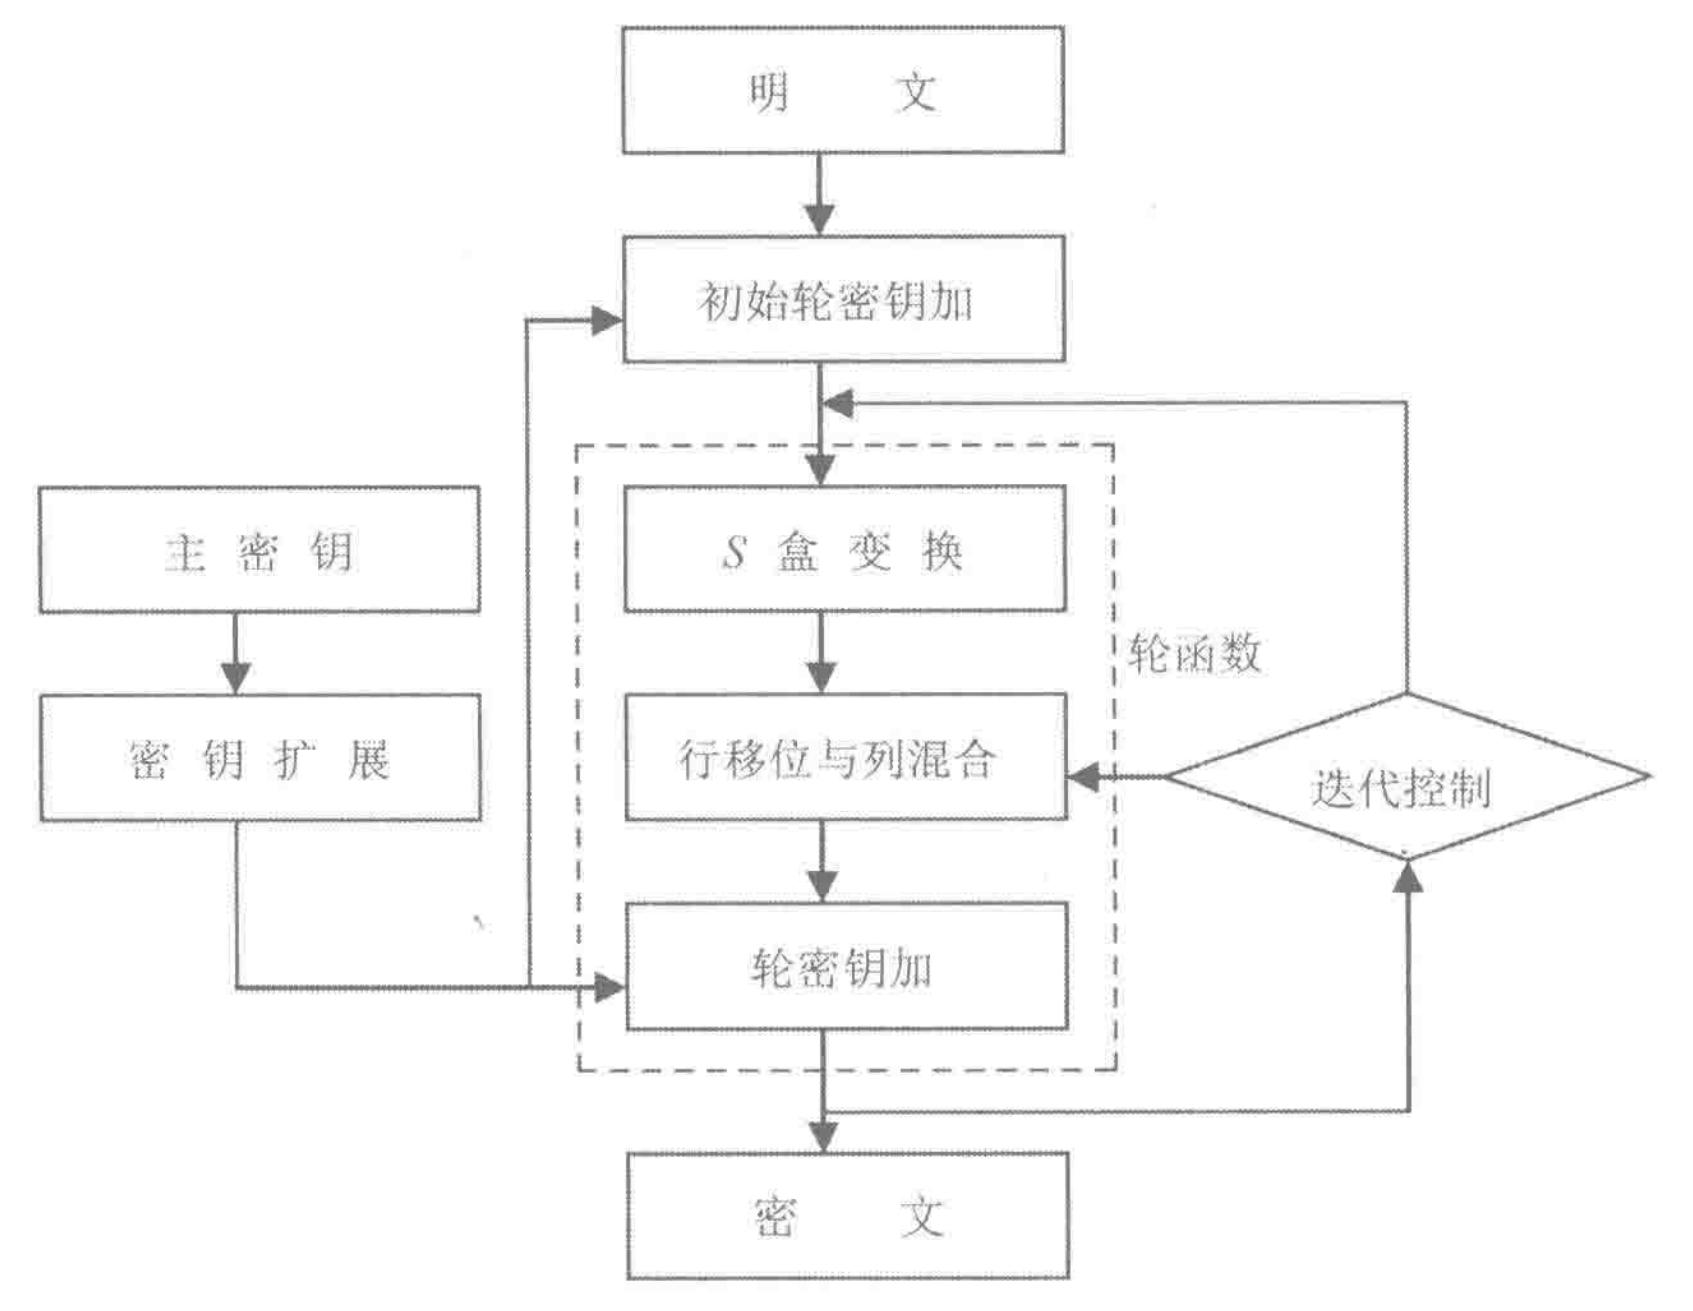
\includegraphics[width=13cm]{AES算法结构.jpg}
                \bottomcaption{\xiaowuhao{AES算法结构}}
            \end{figure}
            明文在经过初始轮密钥加之后进入到轮密钥中迭代一定的次数之后得到密文,
            在轮密钥加步骤中需要的轮密钥需要由主密钥通过密钥拓展得到。\par
            AES加密过程的代码如下所示
            \lstinputlisting[caption={AES整体加密代码},captionpos=b,firstline=16, lastline=32]{E:/Python_code/codes/密码学/lab_2/AES.py}

        \subsubsection{轮函数}
            轮函数由三层结构组成:\par
            (1)非线性层:进行非线性S盒变换ByteSub,由16个S盒并置而成,起到混淆的作用\par
            (2)线性混合层:进行行移位变换ShiftRow和列混合变换MixColumn以确保多轮之上的高度扩散\par
            (3)密钥加层:进行轮密钥加变换AddRoundKey,将轮密钥与中间状态进行异或运算,实现密钥的加密控制作用\par
\newpage
            轮密钥函数算法的结构如下图所示
            \begin{figure}[H]
                \centering
                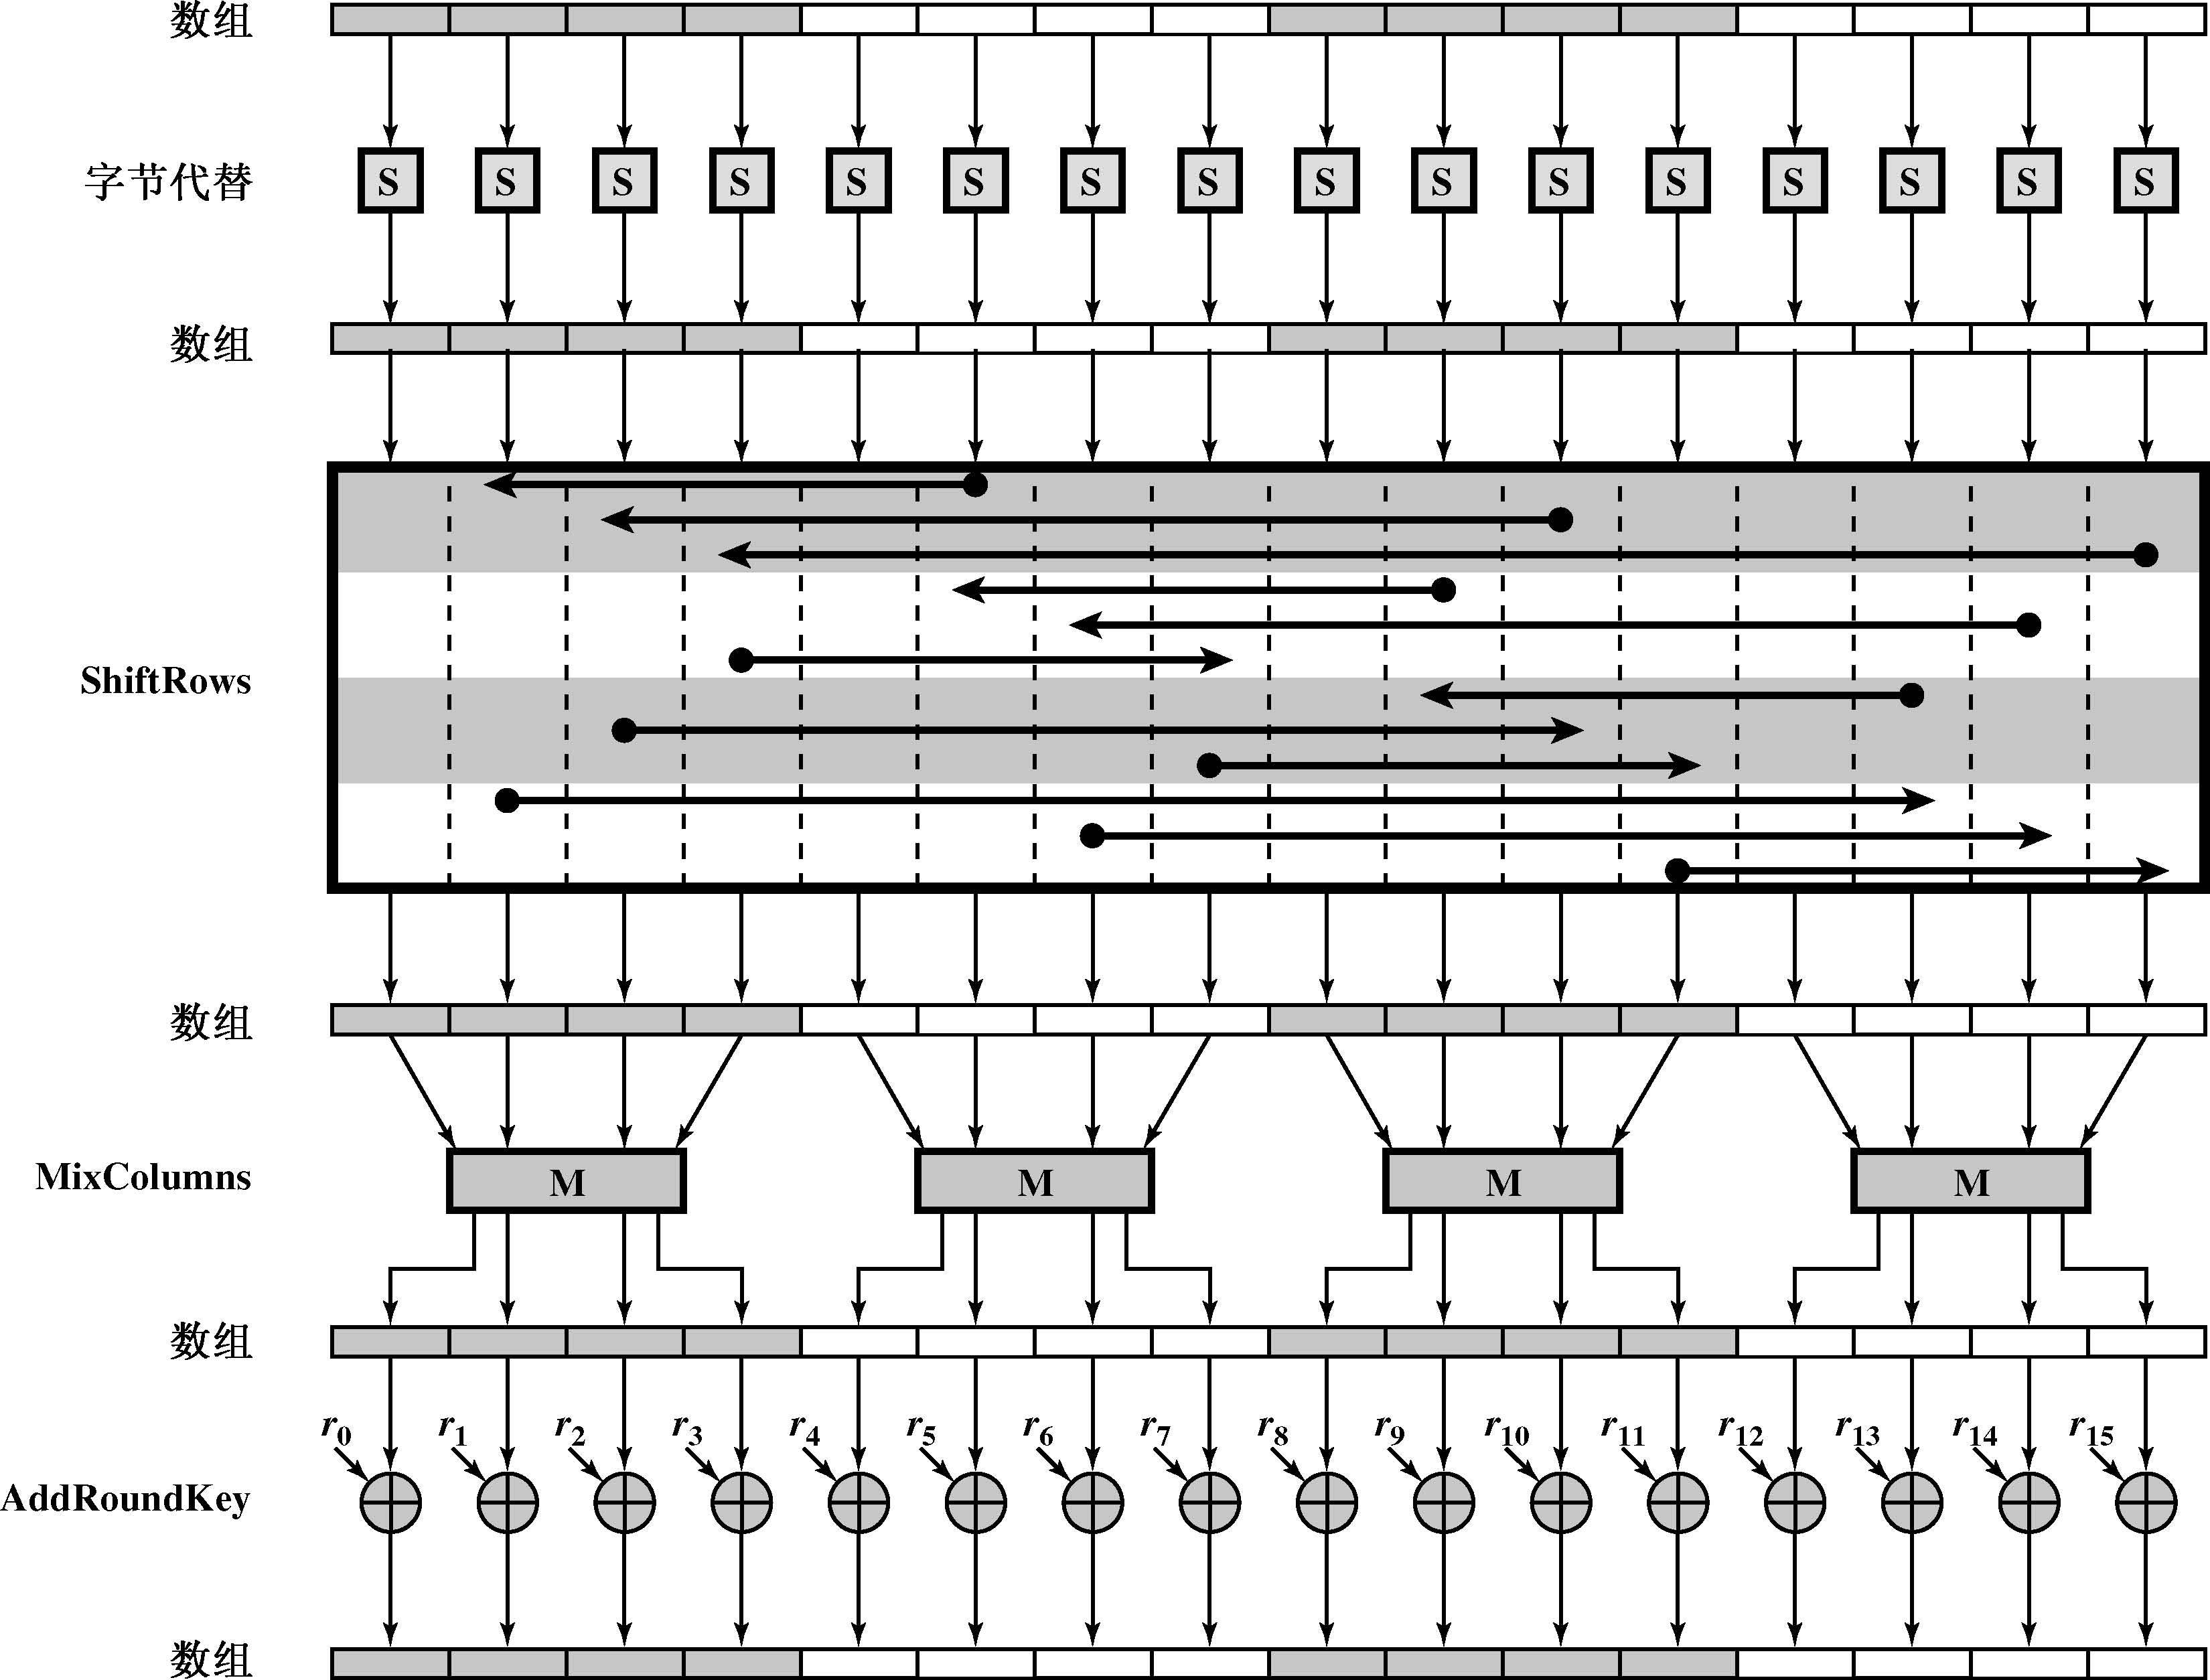
\includegraphics[width=13cm]{轮函数算法结构.png}
                \bottomcaption{\xiaowuhao{轮函数算法结构}}
            \end{figure}
            轮函数的程序代码如下所示
            \lstinputlisting[caption={轮函数代码},captionpos=b,firstline=95, lastline=116]{E:/Python_code/codes/密码学/lab_2/ROUND.py}

        \subsubsection{S盒变换}
            S盒变换是以字节为单位进行代替变换,首先将字节的值用它的乘法逆来代替,其中‘00’的乘法逆为其本身,然后再将处理后的字节
            按照如下图所示的变换公式进行仿射变换
            \begin{figure}[H]
                \centering
                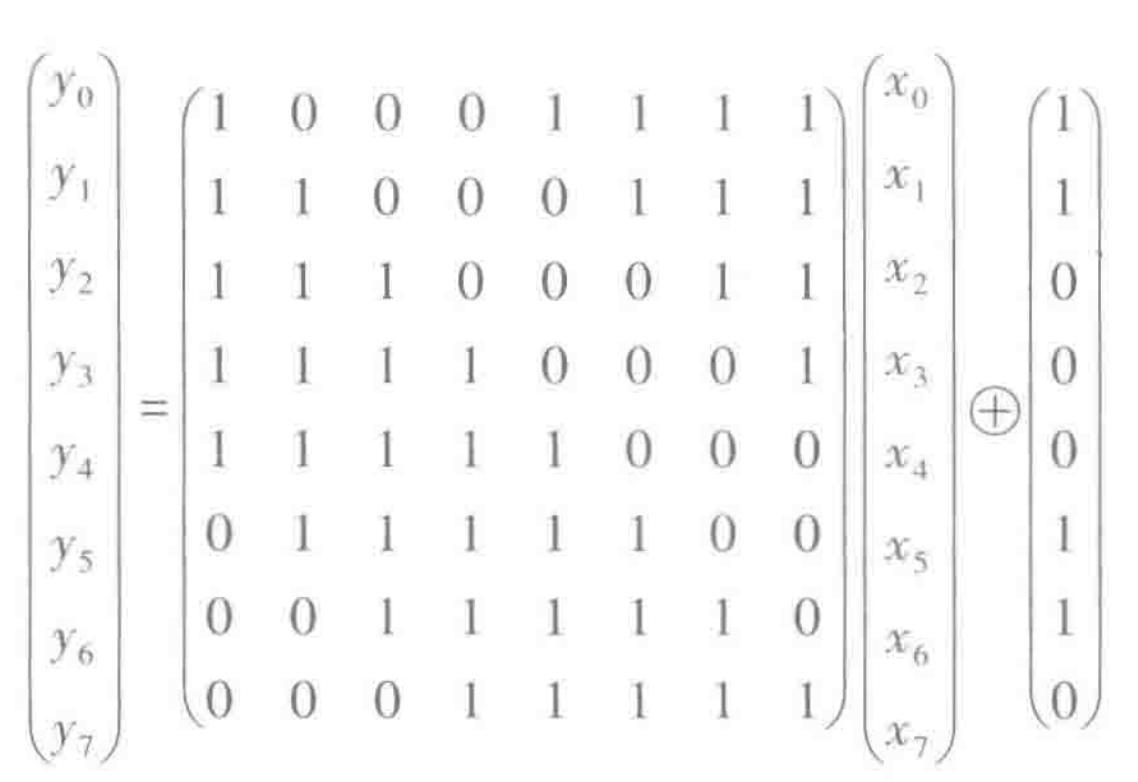
\includegraphics[width=9cm]{S盒仿射变换.jpg}
                \bottomcaption{\xiaowuhao{S盒仿射变换}}
            \end{figure}
        
        \subsubsection{行移位变换ShiftRow}
            行移位变换是将状态的行进行循环左移变换,对于状态的第0行不进行移位操作,对状态的第i行分别循环左移$C[i]$个字节得到行移位变换后的结果
            其中每一行的移位值与Nb有关,其关系如下表所示
            \begin{table}[H]
                \caption{移位值表}\label{tab1}
                  \centering
                \begin{tabular*}{0.75\textwidth}{@{\extracolsep{\fill}}lccc}
                    \toprule
                    Nb          &C1        &C2         &C3                \\
                    \midrule
                    4             &1                    &2          &3                             \\
                    6             &1                     &2           &3                            \\
                    8             &1                       &3            &4                              \\
                    \bottomrule
                \end{tabular*}
              \end{table}
            行移位操作的程序代码如下所示
            \lstinputlisting[caption={行移位代码},captionpos=b,firstline=10, lastline=34]{E:/Python_code/codes/密码学/lab_2/ROUND.py}

        \subsubsection{列混合变换MixColumn}
            列混合变换时对状态的列进行混合变换,把状态中的每一列看作$GF(2^{8})$上的一个多项式,并与一个固定的多项式
            $c(x)='03'x^{3} +'01'x^{2} +'01'x^{1} +'02'$相乘然后模多项式$x^{4} +1$得到列混合变换的结果。
            在本次实验中通过将每一个字节进行如下图所示的变换规则进行多项式乘法得到变换后的多项式。
            \begin{figure}[H]
                \centering
                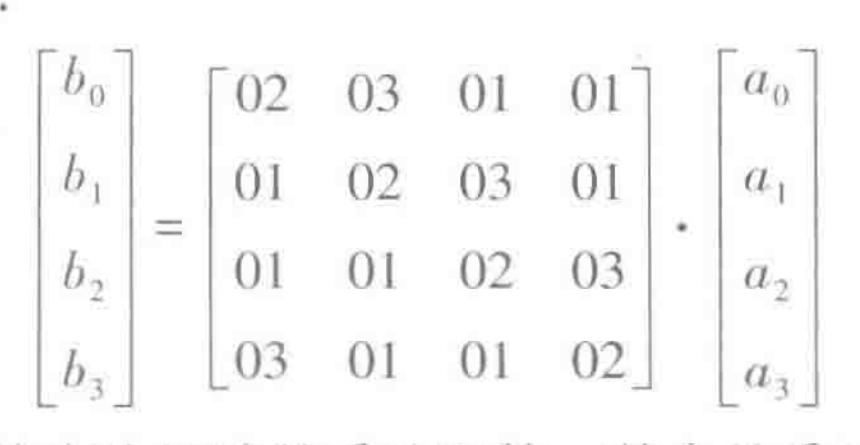
\includegraphics[width=9cm]{列混合变换.jpg}
                \bottomcaption{\xiaowuhao{列混合变换}}
            \end{figure}
            列混合变换的实现代码如下所示
            \lstinputlisting[caption={列混合代码},captionpos=b,firstline=70, lastline=92]{E:/Python_code/codes/密码学/lab_2/ROUND.py}

        \subsubsection{轮密钥加变换AddRoundKey}
            轮密钥加函数主要功能是将当前的轮密钥当作二进制多项式与当前状态进行加和即进行异或操作,其代码如下所示
            \lstinputlisting[caption={轮密钥加代码},captionpos=b,firstline=4, lastline=7]{E:/Python_code/codes/密码学/lab_2/ROUND.py}
              
    \subsection{AES算法的基本运算}

        \subsubsection{$GF(2^{8} )$上的加法与多项式加法}
            在本次实验中由于将状态看作二进制多项式形式并用16进制进行表示,那么两个多项式之间的加法可以看作是
            将其各位进行异或操作,其代码如下所示
            \lstinputlisting[caption={多项式加法代码},captionpos=b,firstline=1, lastline=28]{E:/Python_code/codes/密码学/lab_2/MATH.py}
            首先将得到的两个二进制多项式的字节表示转换成为列表的形式,然后补齐高位后对于每一位进行异或操作,
            最后得到的结果即为两个多项式相加的结果

        \subsubsection{在不同CPU架构下,不同表示方法的执行速度快慢关系}
            (1)数据表示和内存访问模式:\par
                字节级操作:在一些处理器上,如8位或16位微控制器,按字节操作可能更高效,因为这些处理器的数据路径宽度较小。\par
                32位字操作:在32位处理器上,一次处理一个32位的字通常更加高效,因为它可以在单个操作中处理更多的数据。\par
                128位状态操作:在支持SIMD(单指令多数据)指令集的现代处理器(如x86的SSE或ARM的NEON)上,
                可以一次性以128位块的形式处理整个状态,这通常是最快的方法。\par
            (2)CPU指令集:\par
                一些现代处理器拥有专门的指令集和硬件优化,可以一次性处理大量数据。
                例如,支持SIMD(单指令多数据)指令集的处理器可以同时处理多个32位或更大的数据单元。
            (3)CPU位宽:\par
                对于8位或16位微控制器,按字节(8位)操作可能更有效率,因为这些处理器的数据路径和寄存器宽度通常适合较小的数据单元。\par
                对于32位处理器,按字(32位)操作可能更加高效,因为它可以一次处理更多数据,与处理器的自然字大小相匹配。\par
                对于64位处理器,尽管可以有效地执行32位操作,但它们通常能够一次处理更大的数据块,因此可能在某些情况下,按64位操作会更加高效。\par
            (4)内存访问和数据对齐:\par
                在执行异或操作时,内存访问模式也很重要。如果数据没有正确对齐,即数据的内存地址不符合其自然边界,可能会导致性能下降。\par
                一些处理器在处理未对齐的数据时效率较低,这可能会影响按字节或字操作的性能。

        \subsubsection{$GF(2^{8} )$上的乘法}
            (1)借助xtime运算快速实现\par
                借助xtime运算快速实现乘法的代码如下所示
                \lstinputlisting[caption={借助xtime实现多项式加法代码},captionpos=b,firstline=1, lastline=28]{E:/Python_code/codes/密码学/lab_2/disp.py}
                该算法检查b的每一位,如果该位为1,则将a的当前值累加到结果中。同时,a通过应用xtime函数被逐步乘以多项式x,而b则右移一位。
                这个过程持续进行,直到b被完全处理完毕。\par

                该算法的效率分析:\par
                在最好情况下,
                发生在乘数(即b)的二进制表示中只有一个位为1,而其他位都为0。这种情况下,poly\_mul函数只需要进行一次非零位的处理。具体来说:
                如果b是形如00000001的二进制数,那么在第一次迭代中,结果就会直接等于a,后续的迭代中不会再有任何累加,因为b的其他位都是0。
                在这种情况下,函数几乎不需要进行额外的计算,仅需执行一次异或操作和一些基本的位操作,如位移。
                最好情况的时间复杂度是$O(1)$,即常数时间复杂度,因为它几乎不需要进行计算。\par

                在最坏情况下出现在乘数b的所有位都是1,即b是形如11111111的二进制数。在这种情况下,
                每一次迭代中b的当前位都为1,因此函数需要执行最多的异或操作。
                对于a,每次迭代都会执行xtime函数,可能伴随着额外的模约简操作(即异或0x1b)。
                在8次迭代中,每次都需要进行一次异或操作,以及其他的位操作和可能的模约简操作。
                最坏情况的时间复杂度是$O(n)$,其中n是乘数的位数(在这个情况下,n为8),因为它需要对每一位进行处理。\par

            (2)借助生成元实现\par
                借助生成元运算快速实现乘法的代码如下所示
                \lstinputlisting[caption={借助生成元多项式乘法代码},captionpos=b,firstline=29, lastline=49]{E:/Python_code/codes/密码学/lab_2/disp.py}
                首先造表生成有限域 $GF(2^8)$的所有元素。这通常是通过从 0 到 255 的整数表示,并将它们视为多项式的系数。
                构建乘法和加法表,用于快速查找结果。然后查表进行计算:对于多项式乘法中的每一对系数,使用乘法表来获取结果。
                加法相当于二进制下的异或操作(XOR)。最后进行结果合并:将所有的乘法和加法(异或)结果合并,得到最终的多项式乘法结果。

                时间复杂度分析:\par
                首先分析gf\_multiply 函数,这个函数在最坏情况下执行 8 次循环(对应于二进制下 8 位的乘法)。
                在每次循环中,它执行固定数量的操作(赋值、位移、异或等),这些操作的时间复杂度是常数级别的 $O(1)$。
                因此,gf\_multiply 函数的时间复杂度是 $O(8) = O(1)$,即常数时间复杂度。\par
                然后分析polynomial\_multiply 函数,这个函数包含两个嵌套循环,分别对应于两个输入多项式的长度,设为 n 和 m。
                对于每对系数组合,它调用一次 gf\_multiply。因此,总共有 n * m 次 gf\_multiply 调用。\par
                由于 gf\_multiply 是常数时间复杂度,所以 polynomial\_multiply 的总时间复杂度是 $O(n * m)$。
                对于两个长度分别为 n 和 m 的多项式,该算法的时间复杂度是 $O(n * m)$。\par
                空间复杂度分析:\par
                首先分析gf\_multiply 函数,这个函数仅使用了固定数量的局部变量,不依赖于输入大小,因此它的空间复杂度是 $O(1)$。\par
                然后分析polynomial\_multiply 函数,除了输入多项式外,这个函数创建了一个新的数组来存储结果,其长度为 n + m - 1。\par
                因此,polynomial\_multiply 函数的空间复杂度是 $O(n + m)$。该算法的空间复杂度是$ O(n + m)$,
                这是由于它需要存储两个输入多项式和一个长度为 n + m - 1 的结果多项式。

        \subsubsection{$GF(2^{8} )$上的多项式乘法实现}
            在本次实验中采用的多项式乘法的代码如下所示
            \lstinputlisting[caption={多项式乘法代码},captionpos=b,firstline=11, lastline=27]{E:/Python_code/codes/密码学/lab_2/MATH.py}
            在该代码中,函数接收两个十六进制字符串作为输入。然后从十六进制转换为二进制数列表。
            然后初始化一个乘积多项式长度为两个输入列表长度之和减1,然后进行多项式乘法运算,找到多项式a中最高的1位,
            然后遍历多项式b中的每一项,与找到的位进行与操作后异或乘积多项式的对应位置的值即可
        
        \subsubsection{列混合运算实现}
            (1)列混合运算优化1的实现\par
            在列混合运算优化1的算法中,预先计算所有256*6个乘法(01不用计算),这样需要1.5K字节空间,但可省去大量乘法运算,
            其对应的代码如下所示
            \lstinputlisting[caption={列混合优化1代码},captionpos=b,firstline=53, lastline=70]{E:/Python_code/codes/密码学/lab_2/disp.py}

            (2)列混合优化算法2的实现\par
            在该优化算法中,加密算法圈变换中的每一列变换,可通过作4次查表和4次异或运算得到。节省了大量的乘法运算
            \lstinputlisting[caption={列混合优化2代码},captionpos=b,firstline=72, lastline=102]{E:/Python_code/codes/密码学/lab_2/disp.py}
\newpage
            (3)在单片机、手机、PDA等资源受限环境下的实现\par
            在该资源受限的实现算法中,xtime 函数接收一个字节并在有限域$GF(2^{8} )$中将其乘以2,
            如果需要的话会与0x1B进行异或运算以保持结果在域内。mix\_column 函数接收一个四字节的列作为输入,
            并执行列混合操作。这种实现方式不需要预计算表,相比前述的方法,它在存储上更为高效,但在每次操作时需要更多的计算。
            该算法的实现代码如下所示。
            \lstinputlisting[caption={列混合优化2代码},captionpos=b,firstline=105, lastline=126]{E:/Python_code/codes/密码学/lab_2/disp.py}

            时间复杂度分析:\par
            首先分析xtime 函数,该函数执行的是基本的位操作,这些操作的时间复杂度是 $O(1)$,即常数时间。然后分析mix\_column 函数,
            在该函数中,主要操作是几个异或运算和对 xtime 函数的调用。对于每个元素,都执行了一次 xtime 调用和几次异或运算。
            由于这些操作都是常数时间的,所以每个元素的处理时间是常数时间。因此,对于单个四字节的列,mix\_column 函数的时间复杂度是 $O(1)$。\par

            空间复杂度分析:\par
            这两个函数都只使用了固定数量的局部变量。xtime 函数只接受一个字节作为输入,而 mix\_column 函数处理的是一个固定长度为4的字节数组。
            这意味着这两个函数的空间复杂度是 $O(1)$,即它们占用的空间不随输入大小的变化而变化。\par
            因此,该算法的空间复杂度也是 $O(1)$,因为它不需要额外的存储空间,只使用固定数量的局部变量。

            正确性证明:\par
            在证明中通过计算$a[0]$的值对该算法的正确性进行证明。
            在标准运算的列混合中$a'[0]=2*a[0]+3*a[1]+a[2]+a[3]$\par
            而在优化算法中,$a'[0]=a[0]\oplus xtime(a[0]\oplus a[1])\oplus t$\par
            因为$t=a[0]\oplus a[1]\oplus a[2]\oplus a[3]$\par
            所以$a'[0]=a[0]\oplus xtime(a[0]\oplus a[1])\oplus (a[0]\oplus a[1]\oplus a[2]\oplus a[3])$\par
            将xtime展开结果为$a'[0]=a[0]\oplus (2*a[0]\oplus 2*a[1])\oplus a[0]\oplus a[1]\oplus a[2]\oplus a[3]$\par
            简化表达式后得到的结果为$a'[0]=2*a[0]+3*a[1]+a[2]+a[3]$\par
            优化算法与标准算法得到的结果相同,可以证明该优化算法的正确性
            
\section{AES的安全性}
    \subsection{AES的S盒的实现}
        \subsubsection{算法实现}
            在本次实验中为了省去计算S盒的运算时间将S盒变换的结果直接保存到表中,在使用时直接查表得到替换后的字节值
            S盒变换ByteSub部分的代码如下所示
            \lstinputlisting[caption={S盒变换代码},captionpos=b,firstline=100, lastline=124]{E:/Python_code/codes/密码学/lab_2/MATH.py}
        \subsubsection{时间复杂度分析}
            在S盒初始化过程中,S盒是一个固定大小的二维数组(16x16),其初始化时间是常数记位$ O(1)$。在对每个字节的处理中
            函数通过循环遍历输入字节字符串。循环的次数与输入字节的长度成正比。对于每个字节,
            函数执行一系列固定时间的操作(计算行和列索引,然后从S盒中检索相应的值)。
            因此,这部分的时间复杂度与输入字节的长度成正比,即$ O(n)$,其中 n 是输入字节字符串的长度。\par
            由此可见整个S盒变换函数的的总体时间复杂度是$ O(n)$。
            
        \subsubsection{空间复杂度分析}
            S盒是一个固定大小的二维数组,不论输入数据的大小如何,其占用的空间都是常数。所以,这部分的空间复杂度是 $O(1)$。
            对于结果字符串来说其长度与输入字符串 byte 的长度成正比。
            因此,这部分的空间复杂度与输入的长度成正比,即 $O(n)$,其中 n 是输入字节字符串的长度。\par
            所以,整个S盒变换函数的总体空间复杂度也是 $O(n)$。

    \subsection{编程研究AES的S盒的以下特性}

        \subsubsection{明文输入改变1位,密文输出平均改变多少位?}
            将明文输入使用原本的明文,密钥保持不变,每一次改变明文中的一位然后统计密文修改的位数,将得到的密文的改变统计平均值
            编写函数完成这一过程的代码如下所示
            \lstinputlisting[caption={统计密文修改代码},captionpos=b]{E:/Python_code/codes/密码学/lab_2/test_change_m.py}
\newpage
            统计得到的结果如下图所示
            \begin{figure}[H]
                \centering
                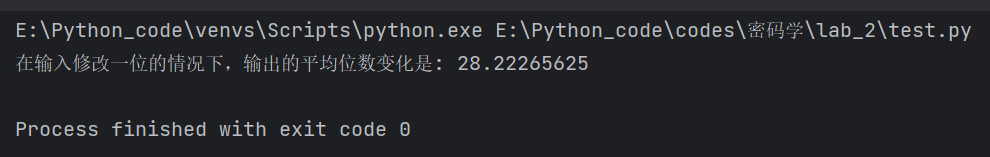
\includegraphics[width=13cm]{change_m.png}
                \bottomcaption{\xiaowuhao{统计密文修改结果}}
            \end{figure}

        \subsubsection{S盒输入改变1位,S盒输出平均改变多少位?}
            将S盒的初始值设置为'a0'每一次改变其中的一位然后统计得到的结果修改的位数,将得到的修改结果统计平均值
            编写函数完成这一过程的代码如下所示
        \lstinputlisting[caption={统计S盒修改代码},captionpos=b]{E:/Python_code/codes/密码学/lab_2/test_change_s.py}
            统计得到的结果如下图所示
            \begin{figure}[H]
                \centering
                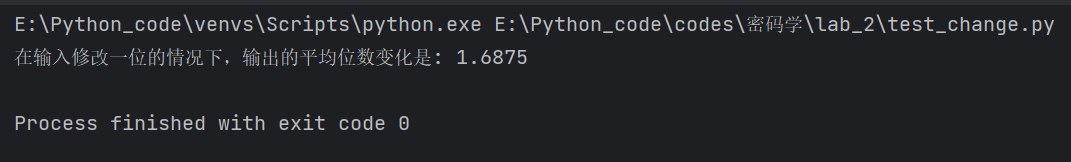
\includegraphics[width=13cm]{change_s.png}
                \bottomcaption{\xiaowuhao{统计密文修改结果}}
            \end{figure}
\newpage
        \subsubsection{对于一个输入,连续施加S盒变换,变换多少次时出现输出等于输入?}
            选取S盒中的每一项作为输入,统计该项经过数次S盒变换得到原值的次数,最后计算总体的平均值
            实现这一步骤的代码如下所示
            \lstinputlisting[caption={统计s盒变换回原值平均值代码},captionpos=b]{E:/Python_code/codes/密码学/lab_2/test_ByteSub.py}
            \begin{figure}[H]
                \centering
                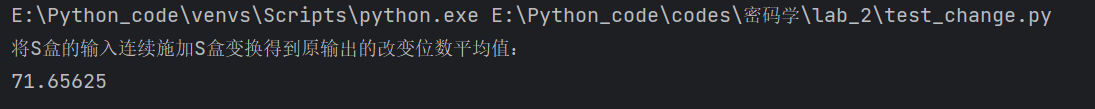
\includegraphics[width=13cm]{s.png}
                \bottomcaption{\xiaowuhao{连续施加s盒结果}}
            \end{figure}
    
\section{拓展思考}
    \subsection{比较AES和DES,说明它们各有什么特点?}
        \subsubsection{AES}
            (1)密钥长度:AES支持128位、192位和256位密钥长度。\par
            (2)安全性:由于较长的密钥长度和更复杂的加密机制,AES比DES提供更高的安全性。它被认为是抵抗所有已知攻击的。\par
            (3)算法结构:AES使用了一个称为Rijndael的加密算法,基于一个称为“状态”的字节矩阵,其加密过程包括多轮的替换、置换和混合操作。\par
            (4)效率:在现代硬件上,AES通常比DES更快,尤其是在处理大量数据时。\par
            (5)应用广泛:AES是目前最流行和最广泛使用的加密标准,用于保护政府、金融机构和其他许多行业的敏感数据。
        \subsubsection{DES}
            (1)密钥长度:DES仅使用56位密钥长度(加上8位奇偶校验,实际长度为64位)。\par
            (2)安全性:由于密钥长度较短,DES容易受到暴力破解攻击。1990年代后期,DES的安全性已经不被普遍认可。\par
            (3)算法结构:DES基于Feistel网络,它通过16轮相同的操作进行加密,每轮使用不同的密钥。\par
            (4)效率:在较老的或资源受限的硬件上,DES可能仍然有效,但它在现代系统中通常比AES慢。\par
            (5)应用范围:虽然现在已经不推荐使用DES,但它在历史上是最广泛使用的加密算法之一,对加密技术的发展有重大影响。

    \subsection{AES的解密算法与加密算法有什么不同?}
        (1)操作顺序:解密过程中的操作是加密过程中操作的逆序。例如,加密中的字节替换在解密时变为逆字节替换。\par
        (2)轮密钥使用:虽然使用的是相同的轮密钥集,但在解密过程中,这些轮密钥的使用顺序与加密过程相反。
        
    \subsection{在$GF(2^8)$中,01的逆元素是什么?}
        由于 '0x01' 本身就是单位元,它与任何多项式相乘的结果都是那个多项式本身。因此,在$GF(2^8)$中,'0x01' 的逆就是它自己,即 '0x01'。

    \subsection{在AES中,对于字节'00'和'01'计算S盒的输出。}
        \subsubsection{'00'}
        (1)求逆元:在$GF(2^8)$中,'00' 没有逆元。对于AES的S盒,当输入是 '00' 时,我们直接跳过求逆元的步骤。\par
        (2)应用仿射变换:对于 '00',仿射变换是简单的,因为不需要与任何值异或。应用AES S盒的固定仿射变换后,
            结果为 '63'。这是因为仿射变换在所有输入为0时输出的固定值。\par
            因此,对于 '00',S盒的输出是 '63'。
        \subsubsection{'01'}
        (1)求逆元:$GF(2^8)$中,'01' 的逆元是它自己,因为任何元素与其逆元相乘的结果为1\par
        (2)应用仿射变换:在找到逆元之后,我们需要对它应用AES S盒的固定仿射变换。仿射变换是一个固定的线性变换,
            通常通过矩阵乘法和向量加法来实现。仿射变换的公式是:\par
            $b(x)=(x\oplus (x\ll 1)\oplus (x\ll 2)\oplus (x\ll 3)\oplus (x\ll 4)\oplus '63') $\par
            其中 $\ll$ 表示循环左移,'63'是十六进制数,对应于二进制的 '01100011'。
            对于'01'(二进制为 '00000001'),\par
            应用上述变换得到:
            $00000001\oplus 00000010\oplus 00000100\oplus 00001000\oplus 00010000\oplus 01100011=01111110$\par
            这个结果是二进制形式,转换为十六进制是 '7E'。
            
    \subsection{证明:模x4+1,$c(x)$与$d(x)$互逆。}
        因为\par
        $c(x)=\left \{ 03 \right \}x^{3}+\left \{ 01 \right \} x^{2}+\left \{  01\right \} x+\left \{ 02 \right \}   $\par
        $d(x)=\left \{ 0B \right \}x^{3}+\left \{ 0D \right \} x^{2}+\left \{  09\right \} x+\left \{ 0E \right \}   $\par
        两个多项式在二进制下表示为\par
        $c(x)=\left (  11\right ) _{2} x^{3}+\left ( 01 \right )_{2}  x^{2}+\left ( 01 \right )_{2}  x+\left ( 10 \right )_{2}  $\par
        $d(x)=\left (  1011\right ) _{2} x^{3}+\left ( 1101 \right )_{2}  x^{2}+\left ( 1001 \right )_{2}  x+\left ( 1110 \right )_{2}   $\par
        将两个二进制多项式直接相乘得到的结果应该为$x^{6}+x^{4}+x^{2}$\par
        与$x^{4}+1$取模之后得到1,得证$c(x),d(x)$互逆
\newpage
    \subsection{证明:xi mod $(x4+1)$=xi mod 4 。}
        对于任意的i,将i分解为i=4k+r的形式,其中r=i mod 4。\par
        将$x^{i}$进行拆分得到$x^{i}=x^{4k+1}=(x^{4})^{k}*x^{r}$\par
        由于$x^{4}\equiv -1 mod (x^{4}+1)$\par
        所以$(x^{4})^{k}*x^{r}$在模$x^{4}+1$的情况下等价于$(-1)^{k}\equiv 1 mod 2$\par
        所以可以得到$x^{i}\equiv x^{r} mod (x^{4}+1)$,又因为r=i mod 4\par
        可以得到结论$x^{i} mod (x^{4}+1)=x^{i mod 4} $

    \subsection{利用AES的对数表或反对数表计算ByteSub$(25)$。}
        首先通过查找AES的对数表和反对数表得到0x25的逆元为0x4d,再将得到的0x4d=01001101进行仿射变换\par
        $y0=(x0+x4+x5+x6+x7)mod 2 \oplus 1 =0$\par
        $y1=(x0+x1+x5+x6+x7)mod 2 \oplus 1=0$\par
        $y2=(x0+x1+x2+x6+x7)mod 2 \oplus 0=1$\par
        $y3=(x0+x1+x2+x3+x7)mod 2 \oplus 0=1$\par
        $y4=(x0+x1+x2+x3+x4)mod 2 \oplus 0=1$\par
        $y5=(x1+x2+x3+x4+x5)mod 2 \oplus 1=1$\par
        $y6=(x2+x3+x4+x5+x6)mod 2 \oplus 1=1$\par
        $y7=(x3+x4+x5+x6+x7)mod 2 \oplus 0=1$\par
        仿射变换后得到S盒的输出为0x3f,所以ByteSub(25)=3f

    \subsection{求出AES的S盒的逆矩阵}
        若S盒的输入为0xXY,则需要在S盒矩阵中查找第X行和第Y列的值,假设得到的S盒的出为0xGH,则根据该S盒构造的逆S盒应当将G行H列位置的元素设置为XY
        以实现求出S盒的逆。计算S盒的逆矩阵的算法如下所示
        \lstinputlisting[caption={计算S盒逆矩阵代码},captionpos=b]{E:/Python_code/codes/密码学/lab_2/test_get_S-1.py}
        算法运行后的结果如下图所示,能够求出给出的S盒的逆矩阵
        \begin{figure}[htbp]
            \begin{minipage}[t]{0.45\linewidth}
                \centering
                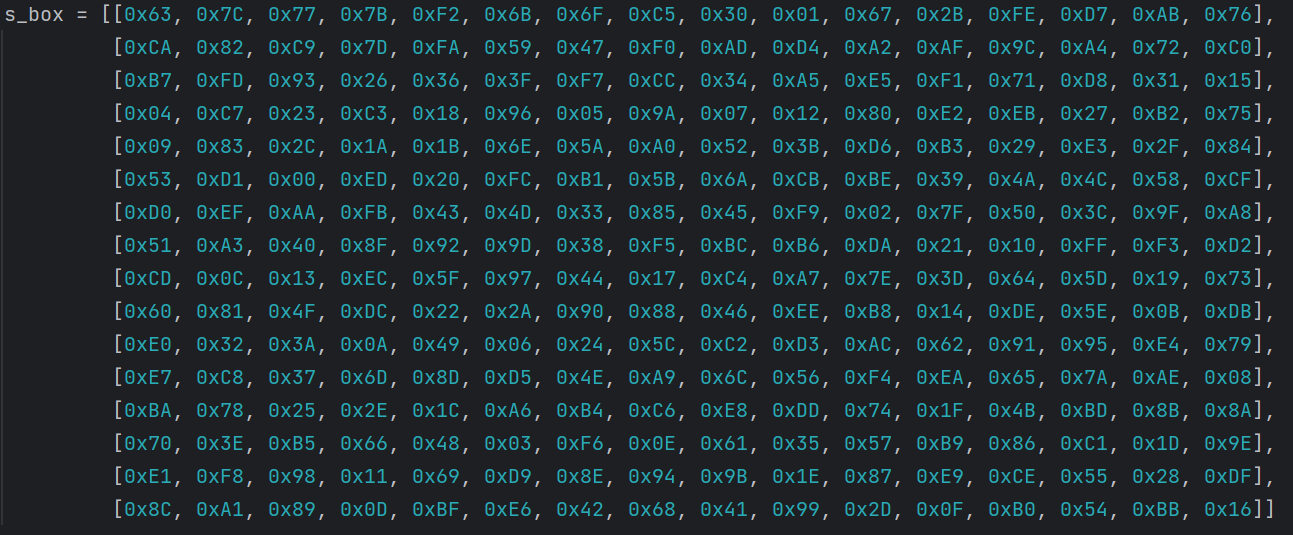
\includegraphics[width=5.5cm,height=3.5cm]{S盒.png}
                \caption{使用的S盒矩阵}
            \end{minipage}
            \begin{minipage}[t]{0.45\linewidth}        %图片占用一行宽度的45%
                \hspace{10pt}
                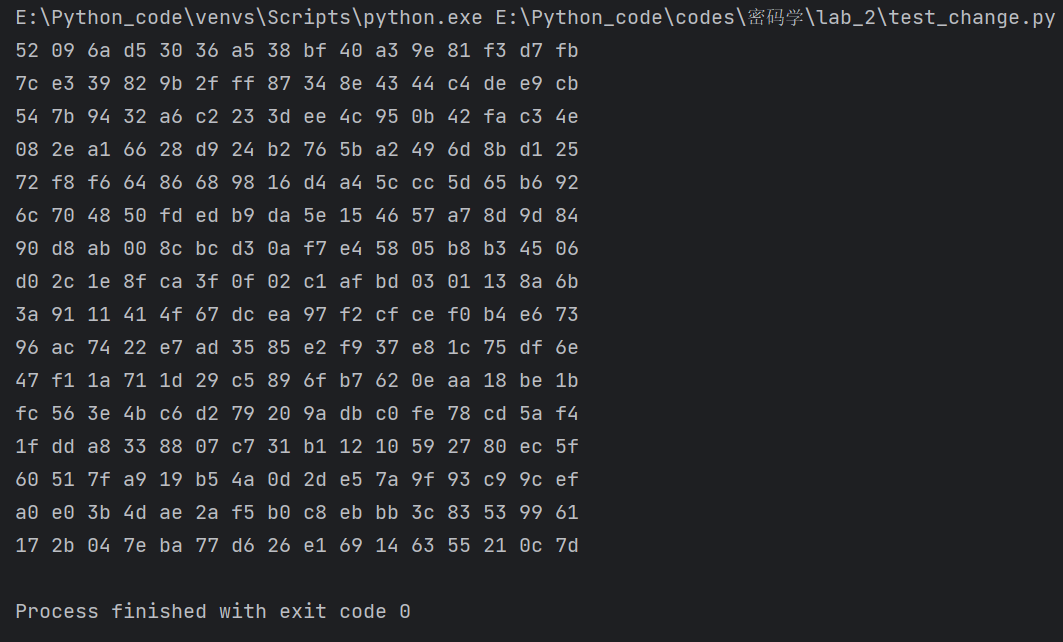
\includegraphics[width=5.5cm,height=3.5cm]{S-1.png}
                \caption{求解出的S盒逆矩阵}
            \end{minipage}
        \end{figure}
        
\newpage
    \subsection{证明}

        \subsubsection{$InvShiftRow(InvByteSub(S))= InvByteSub(InvShiftRow(S))$}
            证明过程如下图所示,两个逆过程的先后并不会影响最终的结果,因为逆行位移会影响到每个字节的位置,
            而逆S变换会影响到每个字节的值,两者并不存在操作顺序的先后关系
            \begin{figure}[H]
                \centering
                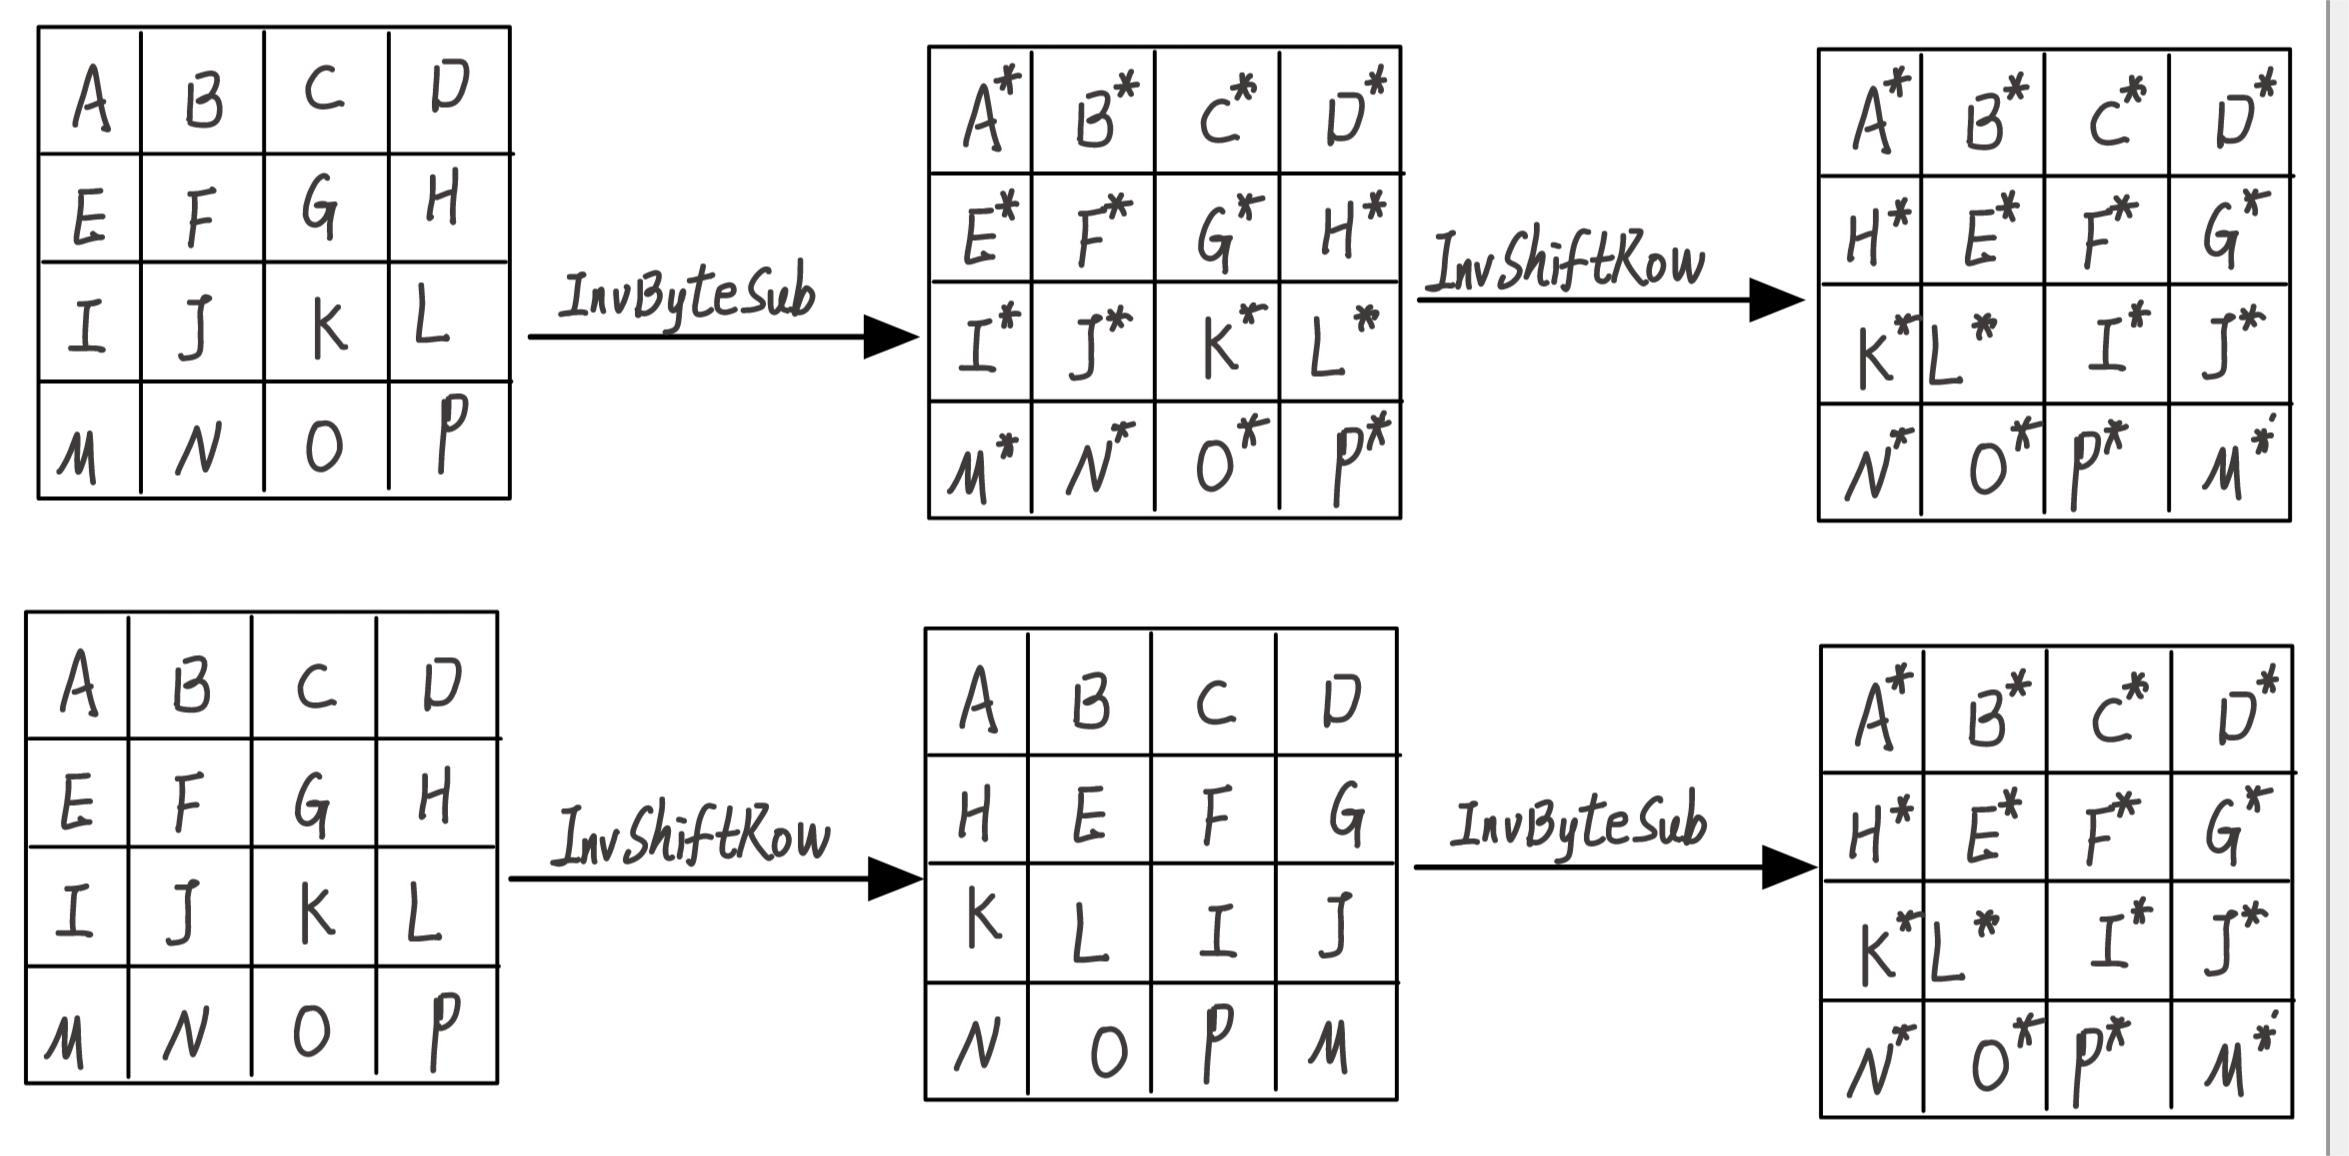
\includegraphics[width=13cm]{证明1.jpg}
                \bottomcaption{\xiaowuhao{证明1}}
            \end{figure}

        \subsubsection{$InvMixColunm(S\oplus W)= InvMixColunm(S)\oplus InvMixColunm(W)$}

            (1)首先,AES算法中的 InvMixColumn操作是矩阵乘法,它对输入矩阵的每一列应用一个特定的线性变换。\par
            (2)将 $S \oplus W$表示为一个新的矩阵 X,即 $X=S\oplus W$\par
            (3)由于 InvMixColumn 操作是线性的,我们可以将等式分解为每一列的等式。对于每一列,我们可以证明 \par
                $InvMixColumn(X_{i})=InvMixColumn(S_{i}) \oplus InvMixColumn(W_{i})$\par
                其中$X_{i},S_{i},W_{i}$分别表示矩阵 X、S和W的第i列\par
            (4)因此,我们得出结论,对于每一列\par
            $InvMixColumn(X_{i})=InvMixColumn(S_{i}) \oplus InvMixColumn(W_{i})$成立\par
            (5)最终,由于这个等式对于矩阵的每一列都成立,我们可以得出整个矩阵的等式:
            $InvMixColumn(X)=InvMixColumn(S) \oplus InvMixColumn(W)$

        \subsubsection{说明上述结论对AES解密算法的设计有何作用}
            (1)算法优化和灵活性:通过这些等式,我们了解到特定的操作步骤可以在不改变最终结果的情况下交换顺序。
                这种灵活性允许算法设计者根据特定的硬件或软件环境调整步骤的执行顺序,以优化性能。
                例如,在某些硬件上,执行顺序的调整可以利用并行处理能力或减少必要的内存访问,从而提高效率。\par
            (2)简化实现:这些数学关系简化了AES解密算法的实现。理解这些等式可以帮助设计者减少算法中的冗余步骤,
                从而减少实现复杂性。这对于需要在资源受限的环境(如嵌入式系统或物联网设备)中实施AES的情况尤为重要。\par
            (3)提高安全性:这些等式还有助于确保算法实现的正确性,这对于保持加密算法的安全性至关重要。
                错误的实现可能会引入安全漏洞。通过确保这些等式在实现中得到正确应用,可以减少由于实现错误导致的安全风险。\par
            (4)可扩展性和可维护性:在软件工程的角度来看,这种数学上的灵活性使得代码更易于维护和扩展。
                例如,如果未来需要对算法进行修改或优化,理解这些基本的数学关系可以帮助设计者在不影响整体安全性和性能的情况下,更容易地进行调整。
            
    \subsection{了解AES采用的SP(代替-置换)结构的特点。}
        (1)层次结构:\par
            SP网络由多个轮(rounds)组成,每一轮都包含一个或多个S-boxes(代替盒子)和P-boxes(置换盒子)。
            在AES中,每个轮包括字节代替、行位移、列混淆和轮密钥加操作。\par
        (2)代替(S-boxes):\par
            S-box是一种非线性替换操作,它将输入的每个字节替换为另一个字节,这种替换基于一个固定的替换表。
            在AES中,S-box用于提供混淆(confusion),即隐藏明文和密文之间的关系。\par
        (3)置换(P-boxes):\par
            P-box是一种线性变换操作,它重新排列或置换输入数据的位。
            在AES中,行位移和列混淆操作共同起到置换的作用,提供扩散(diffusion),即将明文的一个部分分散影响到密文的多个部分。\par
        (4)安全性:\par
            通过将非线性S-boxes和线性P-boxes组合起来,SP网络能够提供很强的抵抗密码分析攻击的能力。
            这种结构有效地破坏了数据的统计结构,使得密码分析变得更加困难。\par
        (5)效率和可实现性:\par
            SP网络特别适合于实现高效的软件和硬件加密算法,因为它们的操作可以并行执行,并且容易转换为电路设计。
            AES特别考虑了在不同平台上(从小型嵌入式设备到大型服务器)的执行效率和实现复杂性。\par

\section{拓展练习}
    \subsection{S盒的安全性测试}
        对于AES S盒,计算其差分分布表和非线性度;\par
        注: 差分分布表的定义是对于一对任意输入x1和x2,满足$\triangle x=x1+ x2$,输出等于$\triangle y=y1+ y2$的统计计数中的最大次数
        例如对于$\triangle x=0$,则$\triangle y=0$出现256次,其余$\triangle y$=1,2,3…,255出现0次,则$\triangle x=0$的差分次数是256;\par
        
        计算差分分布表的代码如下所示
        \lstinputlisting[caption={计算S盒逆矩阵代码},captionpos=b,firstline=5, lastline=35]{E:/Python_code/codes/密码学/lab_2/test_get_ddt.py}
        由于计算得到的差分分布表过长,在这里只展示计算结果的一部分如下图所示
        \begin{figure}[H]
            \centering
            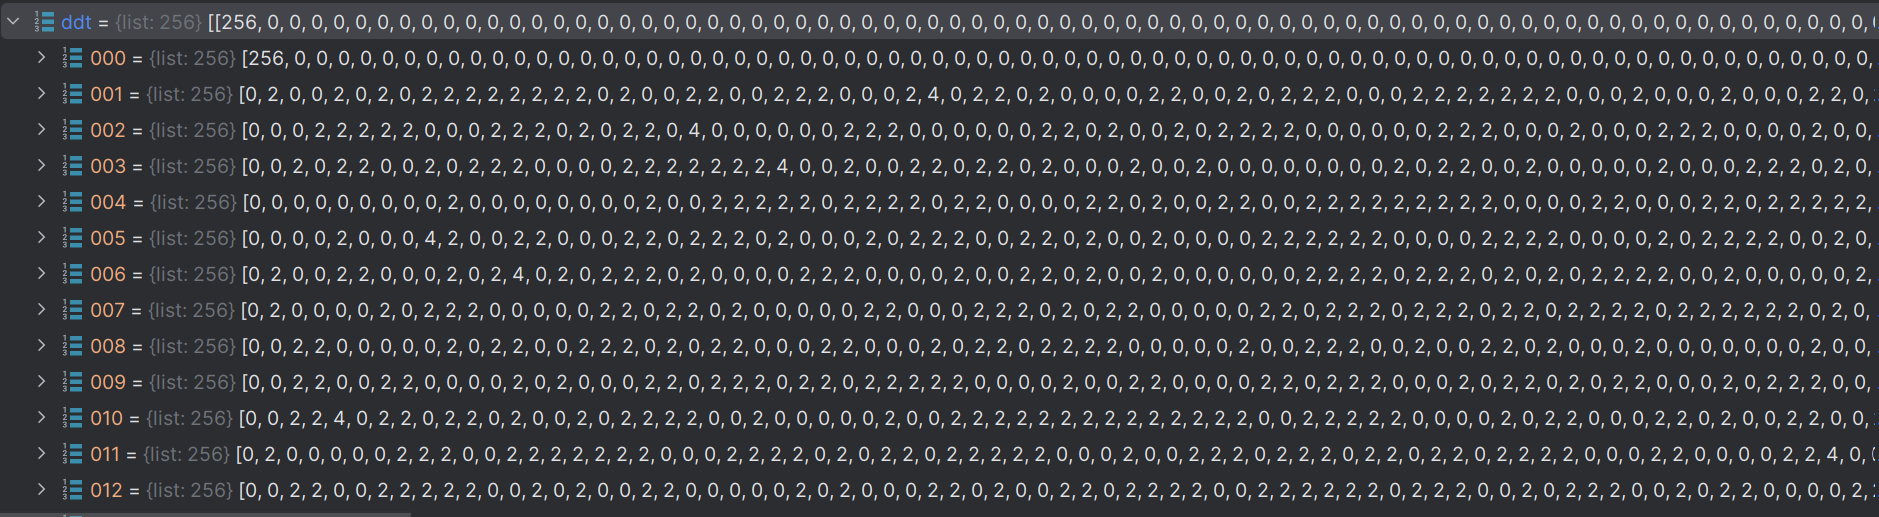
\includegraphics[width=13cm]{差分分布表.png}
            \bottomcaption{\xiaowuhao{差分分布表}}
        \end{figure}

        计算非线性度的代码如下所示
        \lstinputlisting[caption={计算非线性度代码},captionpos=b,firstline=37, lastline=78]{E:/Python_code/codes/密码学/lab_2/test_get_ddt.py}
\newpage
        计算非线性度得到的结果如下图所示
        \begin{figure}[H]
            \centering
            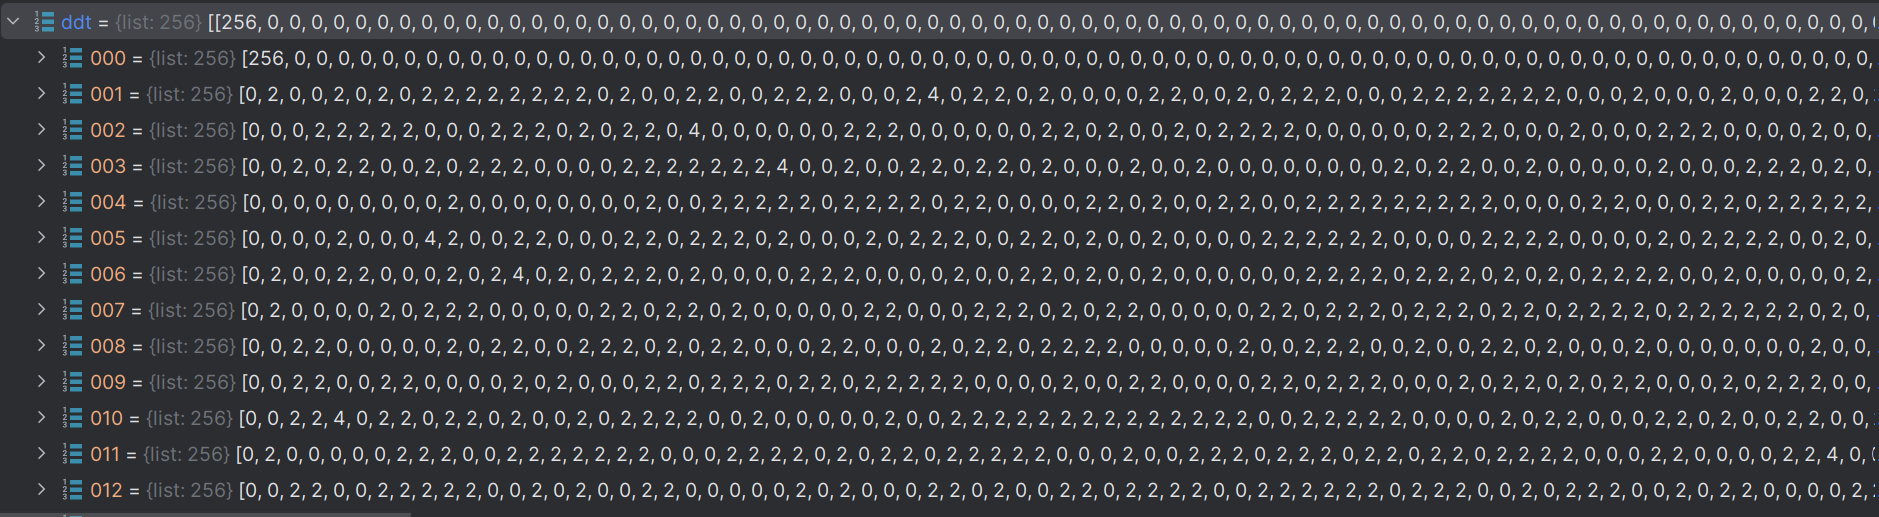
\includegraphics[width=13cm]{差分分布表.png}
            \bottomcaption{\xiaowuhao{差分分布表}}
        \end{figure}

    \subsection{S盒的设计}
        产生新的S盒使其达到题1中的性质最优;
        例:AES的S盒是计算输入X的逆,然后做仿射变换得出输出Y=AX-1+B= AX254+B。
        尝试Y=AXC+B的形式,\par
        (1)C要求汉明重量为7(例如AES中254=11111110),\par
        (2)新盒可以改变仿射变换使用的(满秩)矩阵A或向量B \par
        给出结果,并计算其差分分布表和非线性度。\par
        仅实现了题目一,题目二无法实现

\section{实验结果与数据处理}
    在本次实验中选用的明文为'0001000101a198afda78173486153566',\par
    密钥为'00012001710198aeda79171460153594',程序会将
    明文使用密钥进行加密之后将得到的密文输出,并使用密文运行解密程序,最后将解密得到的明文进行输出,
    程序运行的结果如下图所示
    \begin{figure}[H]
        \centering
        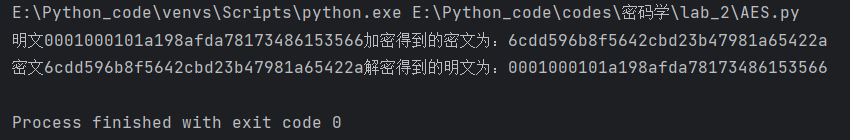
\includegraphics[width=13cm]{result.png}
        \bottomcaption{\xiaowuhao{AES加密解密结果}}
    \end{figure}

\section{分析与讨论}
    (1)深入了解了分组密码的基本概念。分组密码是一种加密算法,它将明文数据分割成固定大小的数据块,
        并通过密钥对每个数据块进行加密和解密。理解了分组密码的工作原理和它在数据加密中的重要性。\par
    (2)全面学习了高级加密标准(AES)密码算法。了解了AES的基本结构,包括轮数、密钥扩展和四个主要操作:
        字节替代、行位移、列混淆和轮密钥加。还学习了AES算法的加密和解密过程,以及如何生成和管理密钥。\par
    (3)讨论了AES密码的安全性。了解了AES被广泛认可为安全可靠的密码算法,其安全性经过了严格的评估和测试。
        学习了AES密码抵抗不同类型的攻击,并了解了为什么它是许多应用中的首选加密算法。\par
    (4)最后熟悉了分组密码的广泛应用。分组密码在网络通信、数据存储、
        安全通信和加密文件等领域都有重要应用。了解了如何在实际应用中使用AES算法来保护数据的机密性和完整性。\par

\section{教师评语}

\end{document}
